\section{Comportamiento del Amplificador Operacional no inversor}

A lo largo de esta sección se procederá a analizar el comportamiento
ideal y real del Amplificador Operacional \emph{LM324 }conectado como
se muestra en la figura \ref{1_b_1}. Considerando los valores de
los componentes como se puede ver en la tabla \ref{1_a_t_1}. 

\begin{figure}[H]
\begin{centering}
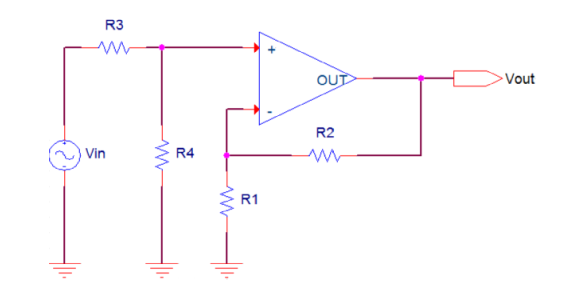
\includegraphics[scale=0.5]{../Ex1/iB/Resources1b/circuit}
\par\end{centering}
\caption{Circuito B}
\label{1_b_1}

\end{figure}

Se implementó en \emph{Altium Designer }como se muestra en las Figuras
\ref{1_b_2} y \ref{1_b_3}.

\begin{figure}[H]
\begin{centering}
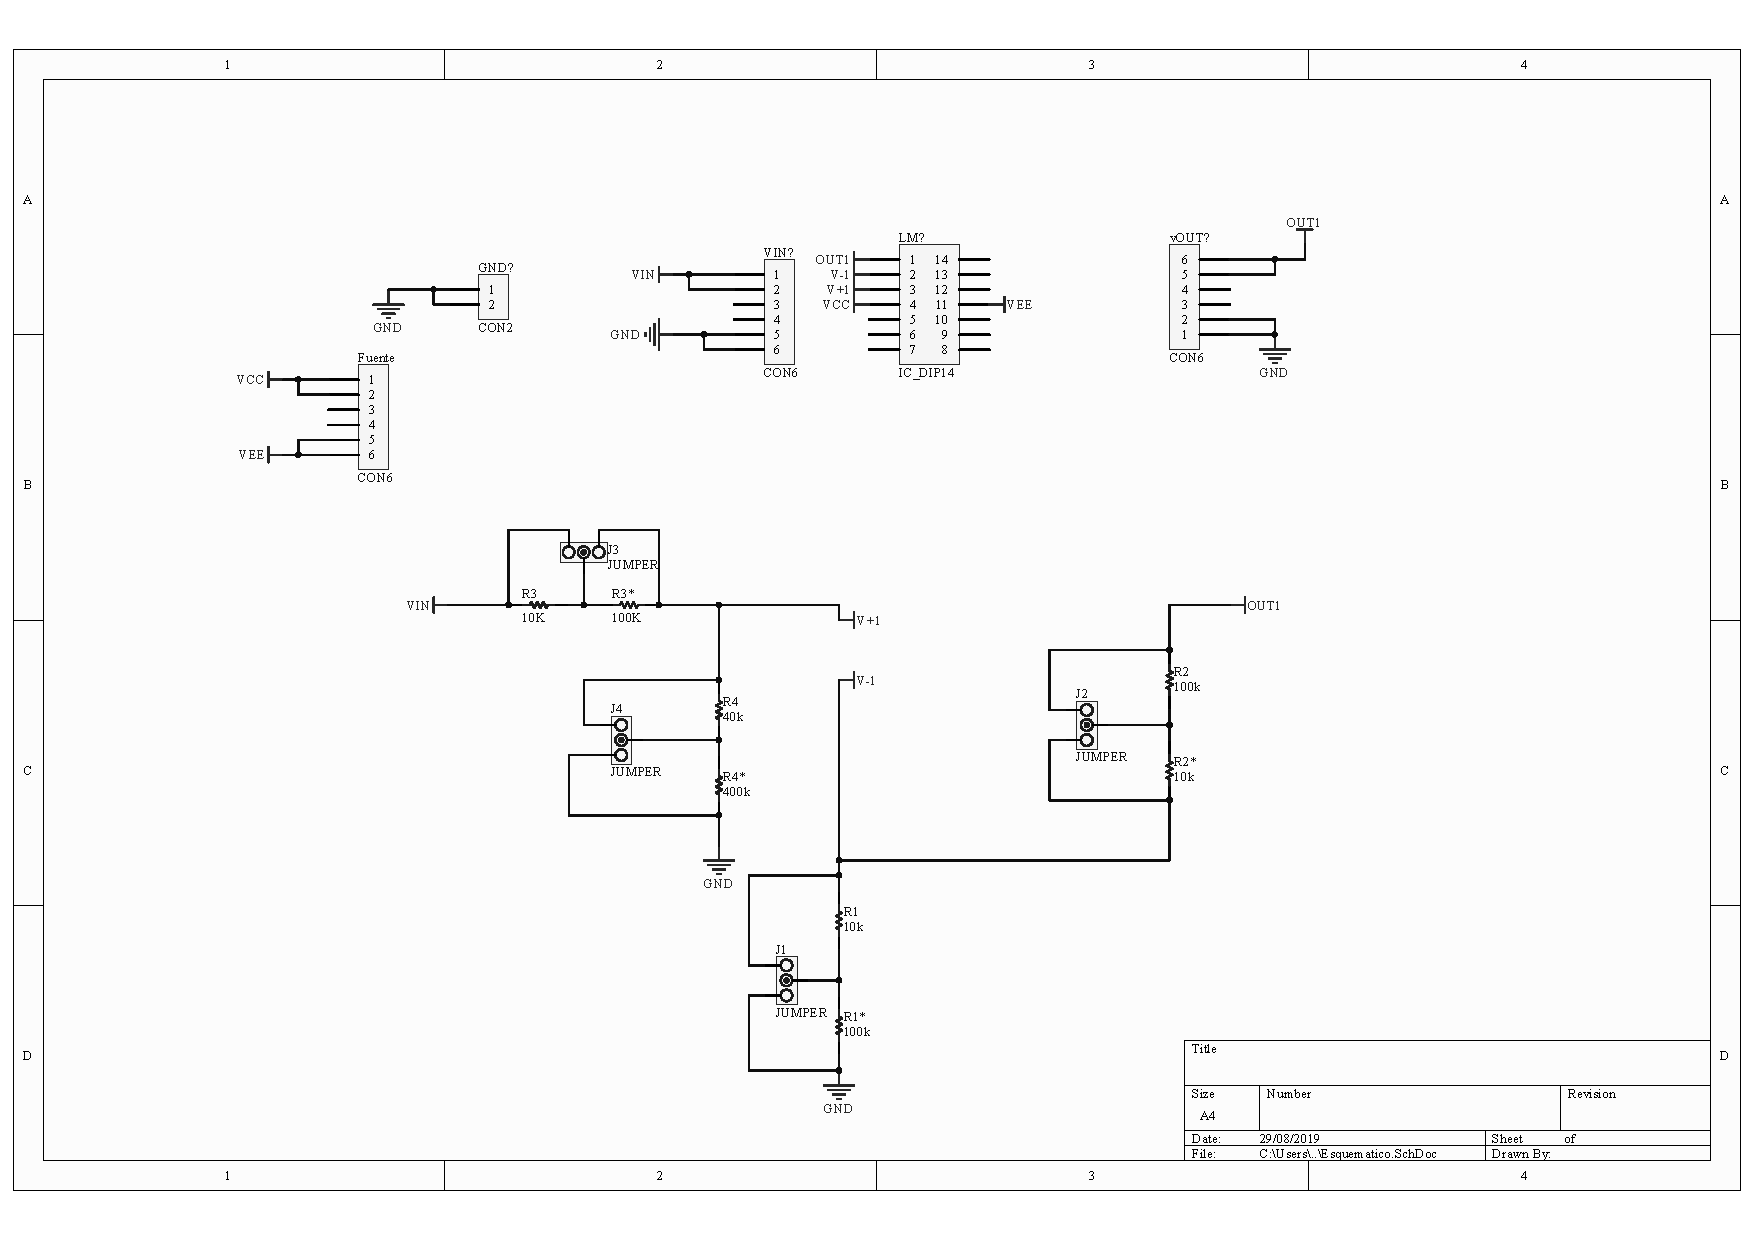
\includegraphics[scale=0.5]{../Ex1/iB/Resources1b/Schematic}
\par\end{centering}
\caption{Esquemático}
\label{1_b_2}

\end{figure}

\begin{figure}[H]
\begin{centering}
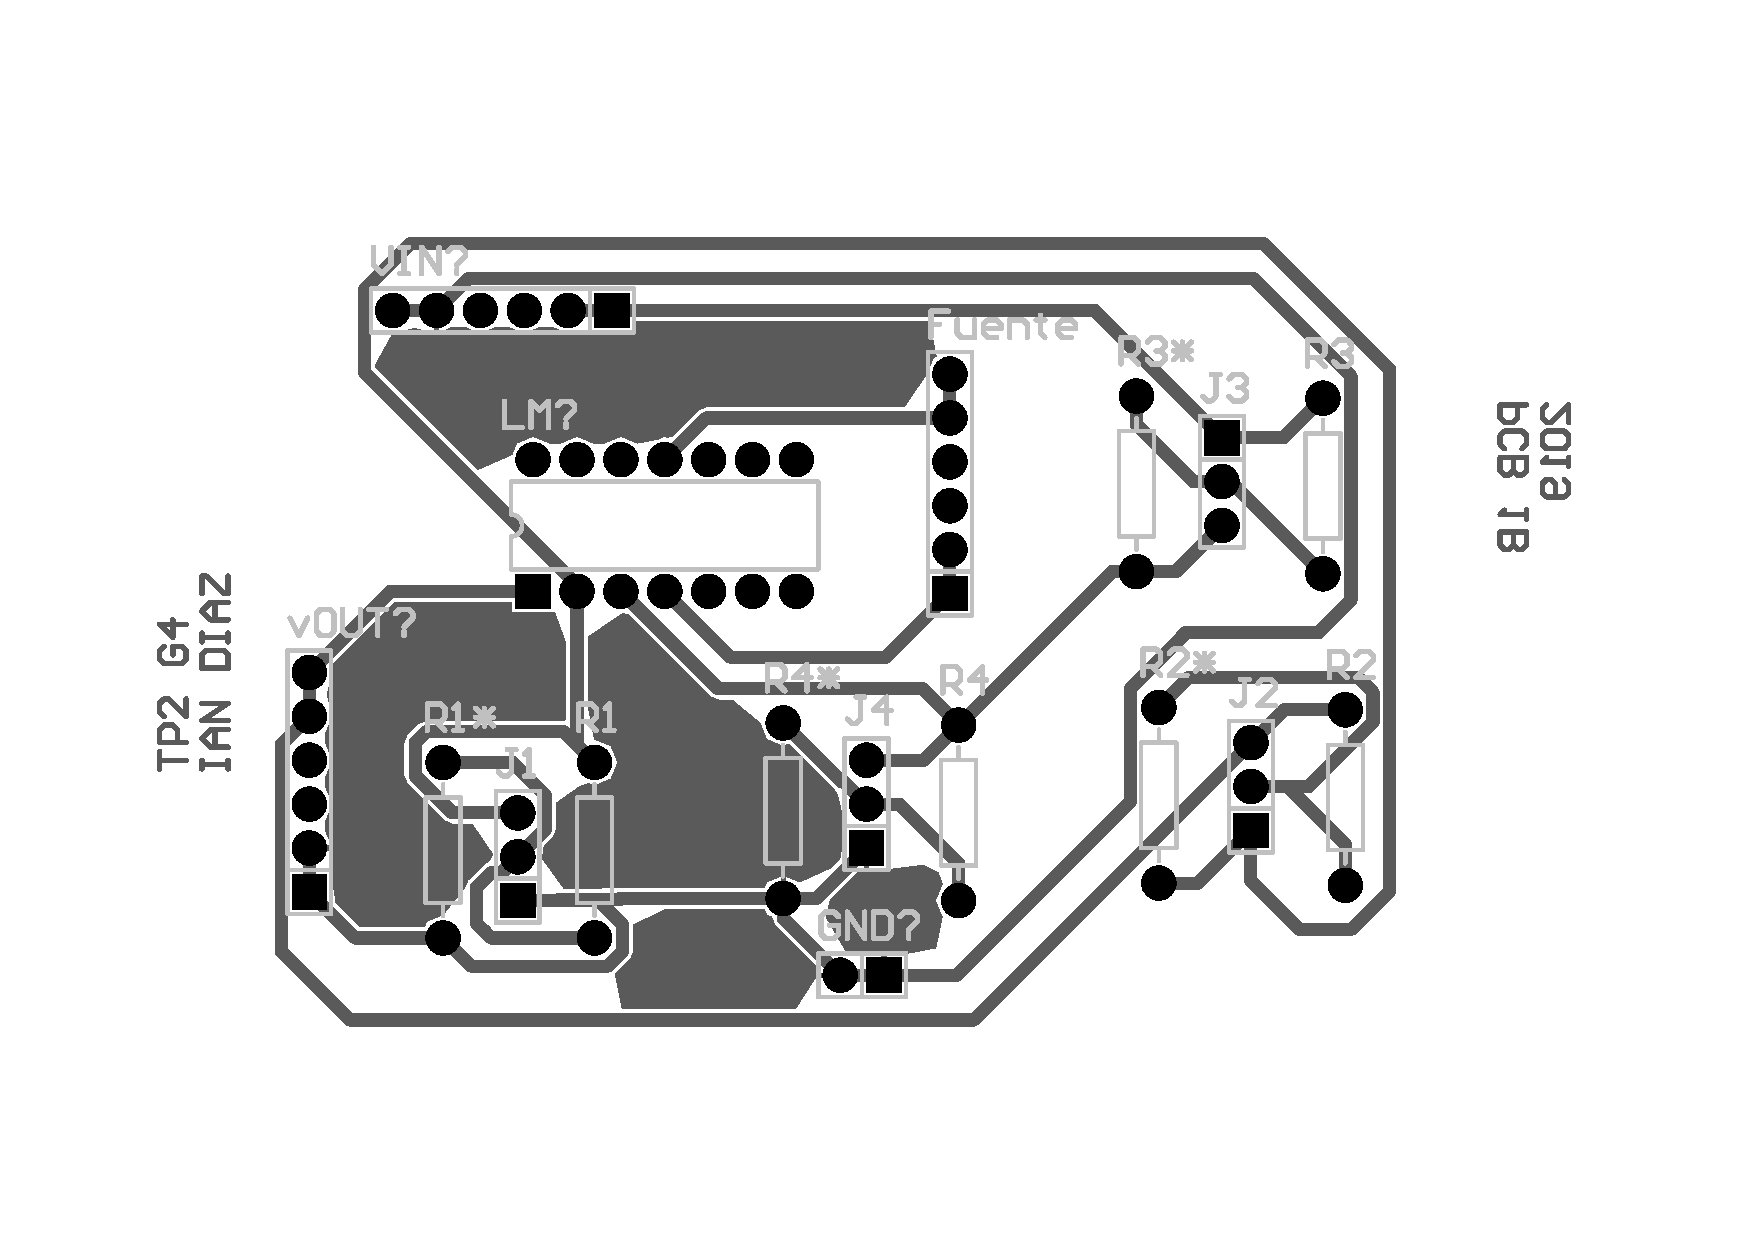
\includegraphics[scale=0.3]{../Ex1/iB/Resources1b/PCB}
\par\end{centering}
\caption{PCB}
\label{1_b_3}

\end{figure}

\subsection{Transferencia}

Comenzando por el análisis ideal, se pidió calcular y graficar la
relación $\frac{V_{out}}{V_{in}}$, esto quiere decir, considerando
$a_{0}$ finito y $A(\omega)$ con polo dominante. Considerando las
siguientes ecuaciones descriptas a continuación y operando correctamente,
se llega a que la relación $\frac{V_{out}}{V_{in}}$ esta dada por
la ecuación (\ref{eq:1_b_1}).

\[
\left\{ \begin{array}{c}
\frac{V_{i}-V^{+}}{R_{3}}=\frac{V^{+}}{R_{4}}\\
\frac{V_{o}-V^{-}}{R_{2}}=\frac{V^{-}}{R_{1}}\\
V_{o}=A(\omega)(V^{+}-V^{-})
\end{array}\right.
\]

\begin{equation}
H(s)=\frac{R_{4}\omega_{p}a_{0}\left(R_{1}+R_{2}\right)}{\left(R_{3}-R_{4}\right)\left(R_{1}\omega_{p}a_{0}+\left(R_{1}+R_{2}\right)\left(\omega_{p}+s\right)\right)}\label{eq:1_b_1}
\end{equation}

\[
H(s)=\frac{414\times10^{9}}{110\times10^{3}s+47\times10^{9}}\,\,\,Caso\,1
\]

\[
H(s)=\frac{75\times10^{9}}{20\times10^{3}s+47\times10^{9}}\,\,\,Caso\,2
\]

\[
H(s)=\frac{414\times10^{9}}{110\times10^{3}s+471\times10^{9}}\,\,\,Caso\,3
\]

\begin{figure}[H]
\begin{centering}
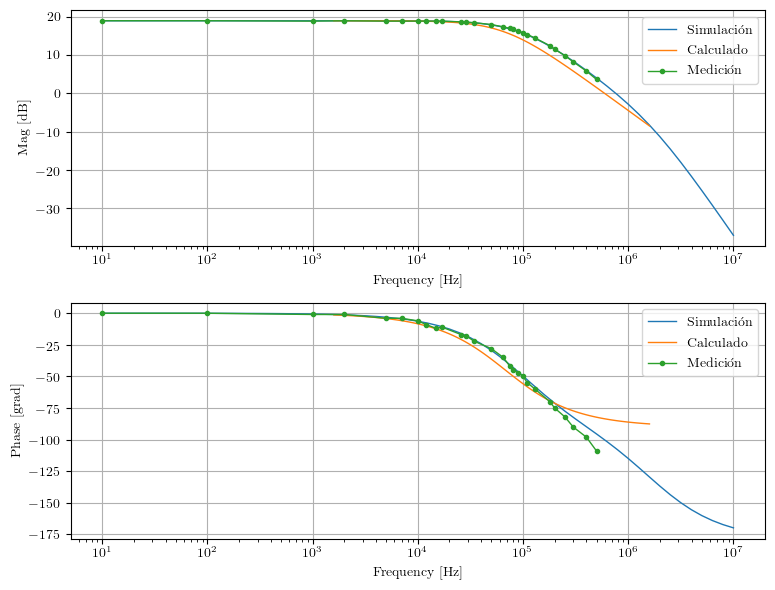
\includegraphics[scale=0.5]{../Ex1/iB/Resources1b/H1b}
\par\end{centering}
\caption{Comportamiento del circuito para el caso 1}
\end{figure}

\begin{figure}[H]
\begin{centering}
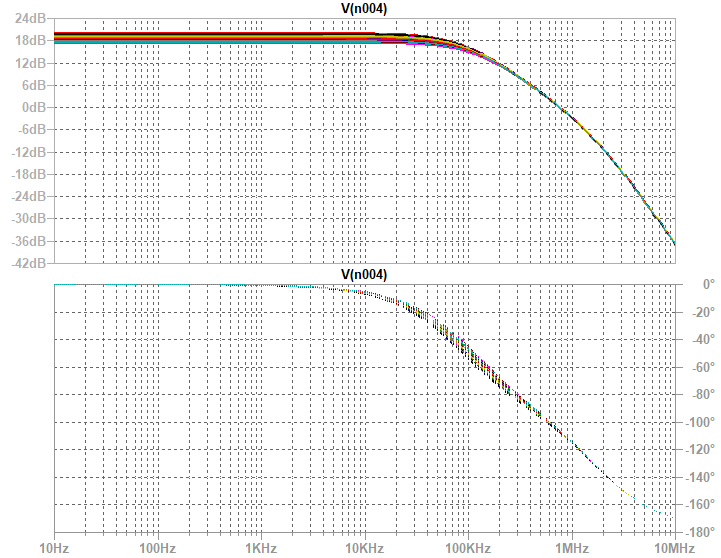
\includegraphics[scale=0.5]{../Ex1/iB/Resources1b/Montecarlo1}
\par\end{centering}
\caption{Análisis montecarlo del caso 1}
\end{figure}

\begin{figure}[H]
\begin{centering}
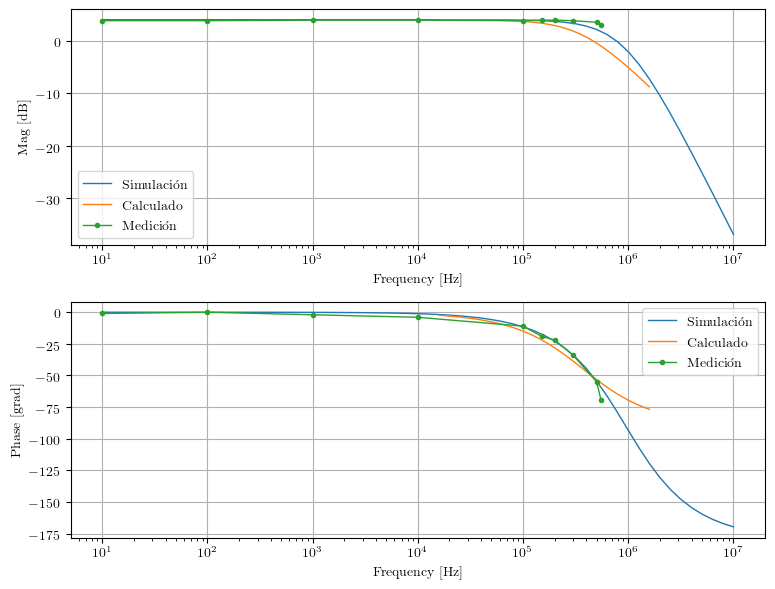
\includegraphics[scale=0.5]{../Ex1/iB/Resources1b/H2b}
\par\end{centering}
\caption{Comportamiento del circuito para el caso 2}
\end{figure}

\begin{figure}[H]
\begin{centering}
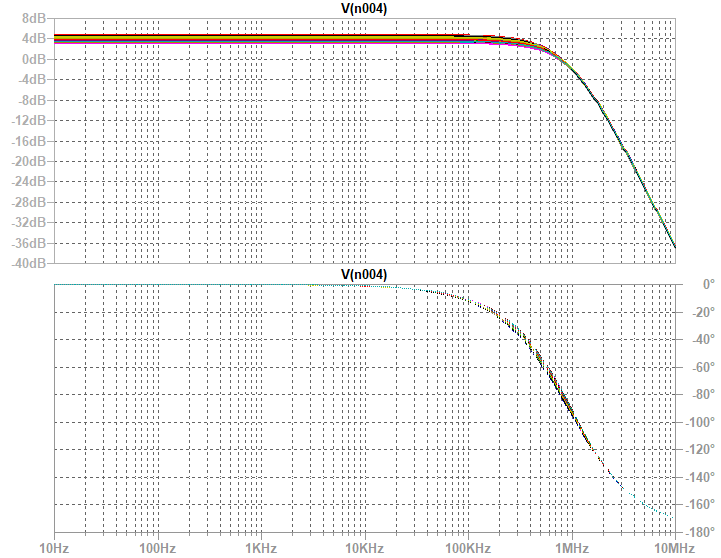
\includegraphics[scale=0.5]{../Ex1/iB/Resources1b/Montecarlo2}
\par\end{centering}
\caption{Análisis montecarlo del caso 2}
\end{figure}

\begin{figure}[H]
\begin{centering}
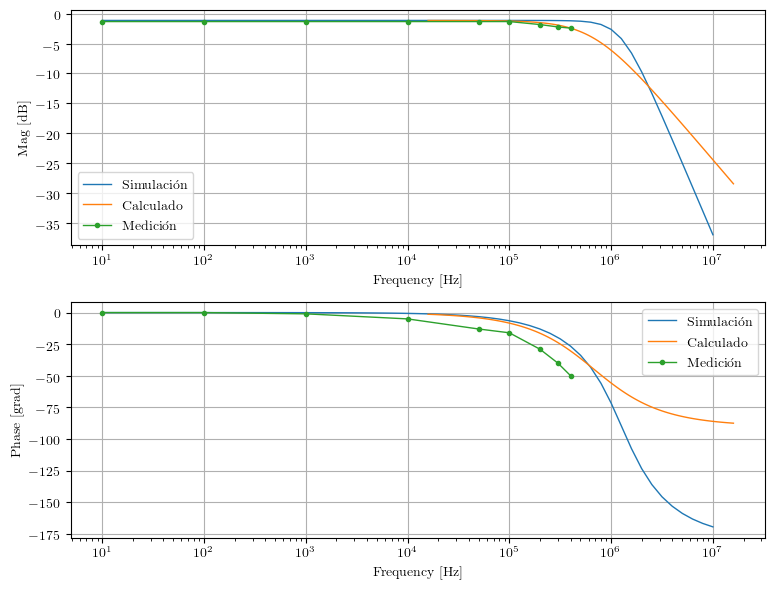
\includegraphics[scale=0.5]{../Ex1/iB/Resources1b/H3b}
\par\end{centering}
\caption{Comportamiento del circuito para el caso 3}
\end{figure}

\begin{figure}[H]
\begin{centering}
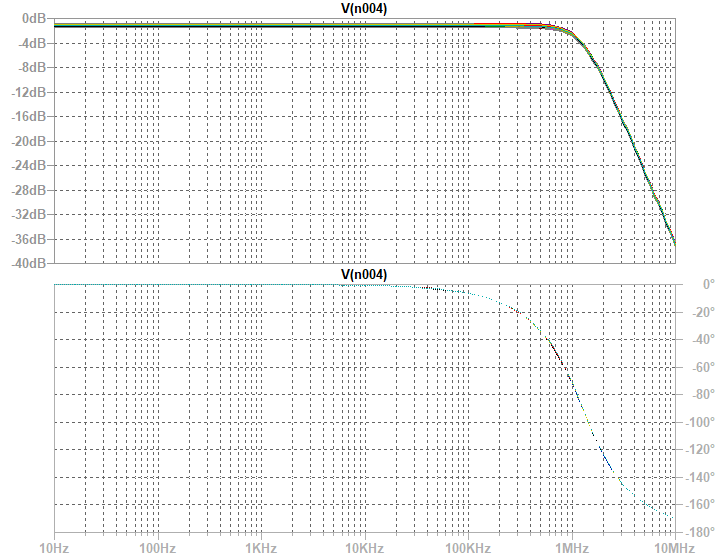
\includegraphics[scale=0.5]{../Ex1/iB/Resources1b/Montecarlo3}
\par\end{centering}
\caption{Análisis montecarlo del caso 3}
\end{figure}

Como se puede observar, los circuitos siguen, dentro de los parámetros
adecuados, y considerando capacidades, inductancias y resistencias
parásitas, las simulaciones y la transferencia calculada. Las diferencias
entre la transferencia calculada y la simulacón se deben a las puntas
de los osciloscopios, que me generan polos de 2do orden, sumados a
los polos de los capacitores internos a los transistores de juntura
bipolar, que provocan que la pendiente de atenuacion de nuestro circuito
se mayor a la calculada, y a su vez, que el cambio de fase no sea
de 90\textdegree , sino de 180\textdegree .

\subsection{Impedancia de entrada}

Consecuentemente, se nos instó a calcular la impedancia de entrada
vista por el generador hacia nuestro circuito. Nuevamente, se utilizo
el \emph{Circuit Solver }creado en Python para calcular las expresiones
de las impedancias de entrada. La ecuación que describe la impedancia
de entrada se detalla en la ecuación (\ref{eq:1_b_2}).

\begin{equation}
Z_{inp}=R_{3}+R_{4}\label{eq:1_b_2}
\end{equation}

Por lo tanto, las impedancias de entrada para cada caso serán;

\[
Z_{inp}=50(k\Omega)\,\,\,Caso\,1
\]

\[
Z_{inp}=50(k\Omega)\,\,\,Caso\,2
\]

\[
Z_{inp}=500(k\Omega)\,\,\,Caso\,3
\]

Teniendo en cuenta estos resultado, y a diferencia de lo visto previamente
en el análisis del circuito inversor, se puede observar como la impedancia
de entrada permanece constante frente a cambios de frecuencia en la
tensión de entrada.

\begin{figure}[H]
\begin{centering}
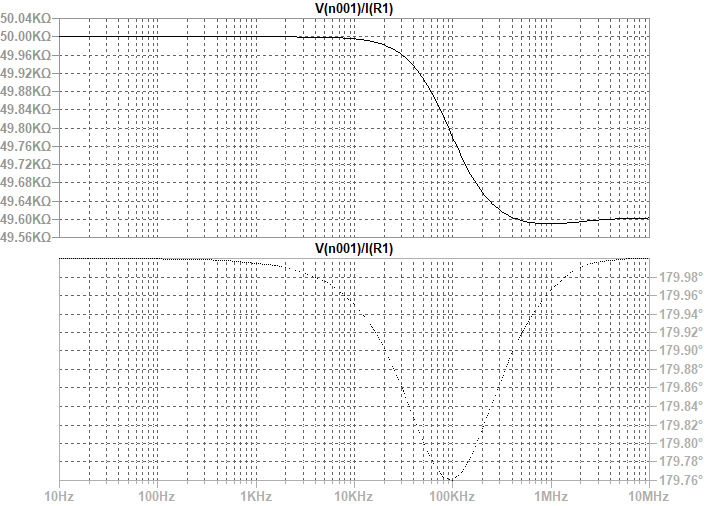
\includegraphics[scale=0.5]{../Ex1/iB/Resources1b/zinp1_sim}
\par\end{centering}
\caption{Simulación de la impedancia de entrada para el caso 1}

\end{figure}

\begin{figure}[H]
\begin{centering}
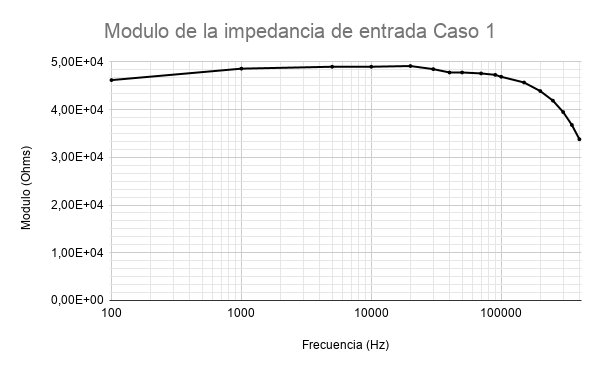
\includegraphics[scale=0.4]{../Ex1/iB/Resources1b/zinp1_m_med}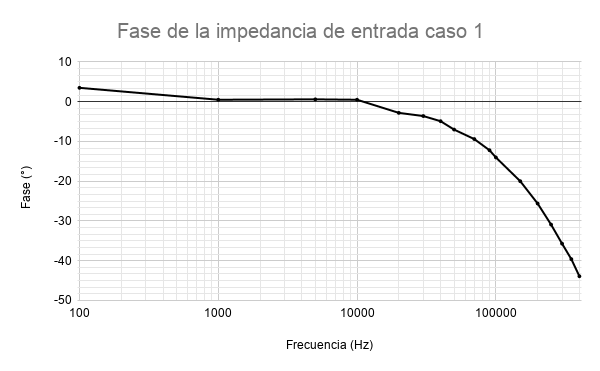
\includegraphics[scale=0.4]{../Ex1/iB/Resources1b/zinp1_p_med}
\par\end{centering}
\caption{Medición de la impedancia de entrada para el caso 1}

\end{figure}

\begin{figure}[H]
\begin{centering}
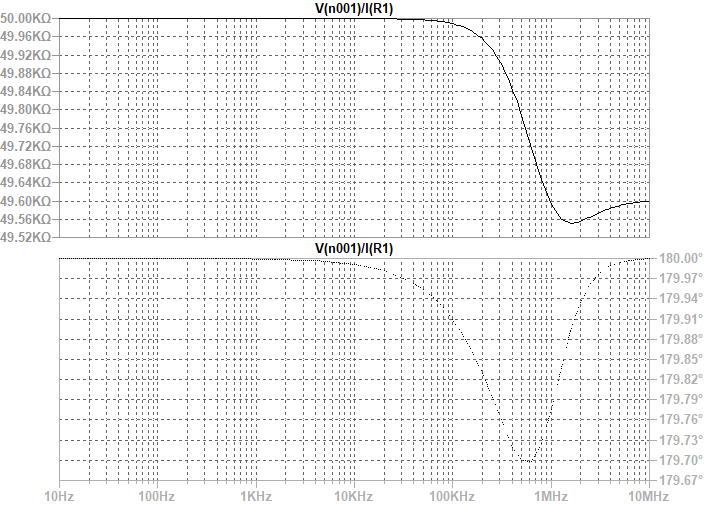
\includegraphics[scale=0.5]{../Ex1/iB/Resources1b/zinp2_sim}
\par\end{centering}
\caption{Simulación de la impedancia de entrada para el caso 2}
\end{figure}

\begin{figure}[H]
\begin{centering}
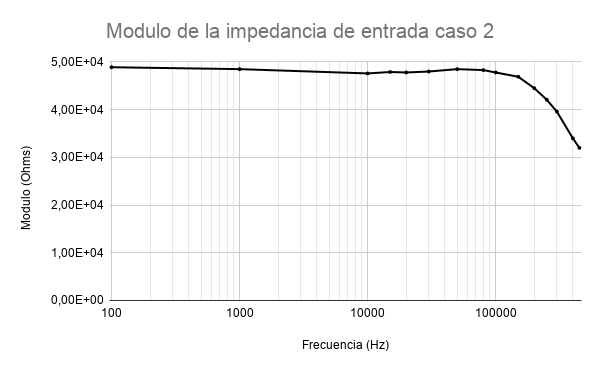
\includegraphics[scale=0.4]{../Ex1/iB/Resources1b/zinp2_m_med}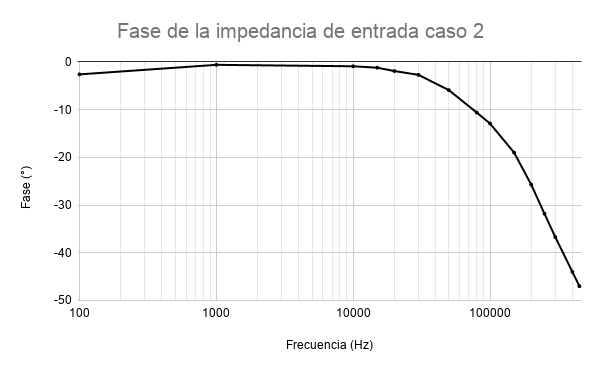
\includegraphics[scale=0.4]{../Ex1/iB/Resources1b/zinp2_p_med}
\par\end{centering}
\caption{Medición de la impedancia de entrada para el caso 2}
\end{figure}

\begin{figure}[H]
\begin{centering}
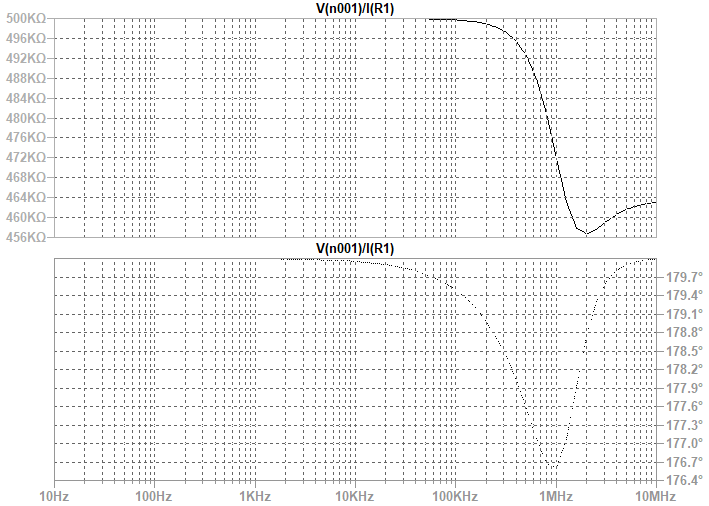
\includegraphics[scale=0.5]{../Ex1/iB/Resources1b/zinp3_sim}
\par\end{centering}
\caption{Simulación de la impedancia de entrada para el caso 3}
\end{figure}

\begin{figure}[H]
\begin{centering}
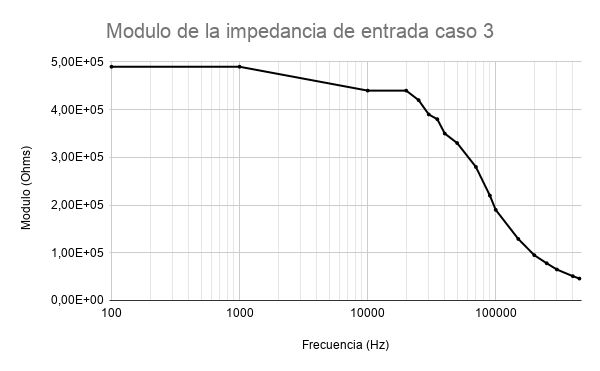
\includegraphics[scale=0.4]{../Ex1/iB/Resources1b/zinp3_m_med}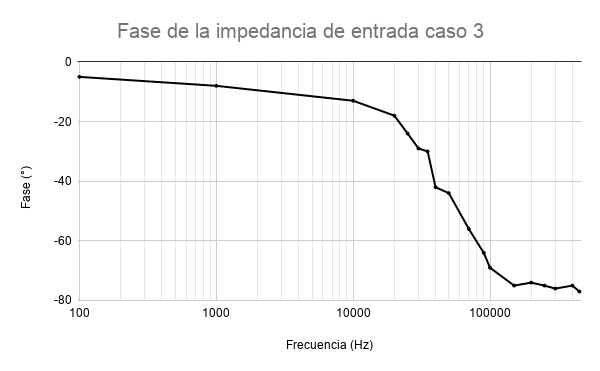
\includegraphics[scale=0.4]{../Ex1/iB/Resources1b/zinp3_p_med}
\par\end{centering}
\caption{Medición de la impedancia de entrada para el caso 3}
\end{figure}

Observando los graficos de las simulaciones y comparandolos con la
ecuación (\ref{eq:1_b_2}), se puede observar como practicamente la
impedancia de entrada permanece constante para todas las frecuencias.
El hecho de que la impedancia de entrada tenga una pequeña variación
en modulo y fase en la simulación, se debe a que para hacer el analisis
de la impedancia de entrada se consideró el Amplificador Operacional
ideal, es decir, $R_{id}\longrightarrow\infty$ y $R_{o}\longrightarrow0$,
por lo tanto, no se tienen en cuenta el efecto de esas resistencias,
como a su vez sus inductancias y capacidades intrínsecas del amplificador.
Sin embargo, considerando la ecuación propuesta, y observando los
resultados simulado, se puede observar que prácticamente no hay problema
en aproximar la impedancia de entrada como constante en ninguno de
los 3 casos (Considerando un 10\% de error en el ultimo caso).

Por otro lado, si analizamos las mediciones, podemos ver que para
frecuencias mayores a 10(kHz), el modelo se aleja bastante de los
resultados empíricos. Esto se explica debido a las capacidades parásitas
que se generaron a la hora de medir la impedancia de entrada, que
considerando a $Z_{inp}=R_{3}+R_{4}$, me generan un circuito pasabajos
de primer orden, obteniendo así los resultados vistos en las mediciones.
Si simulamos nuestro circuito, considerando las capacidades parásitas,
comienza a ser observable el efecto pasabajos que se genera, y se
pone en evidencia los resultados empíricos.

\begin{figure}[H]
\begin{centering}
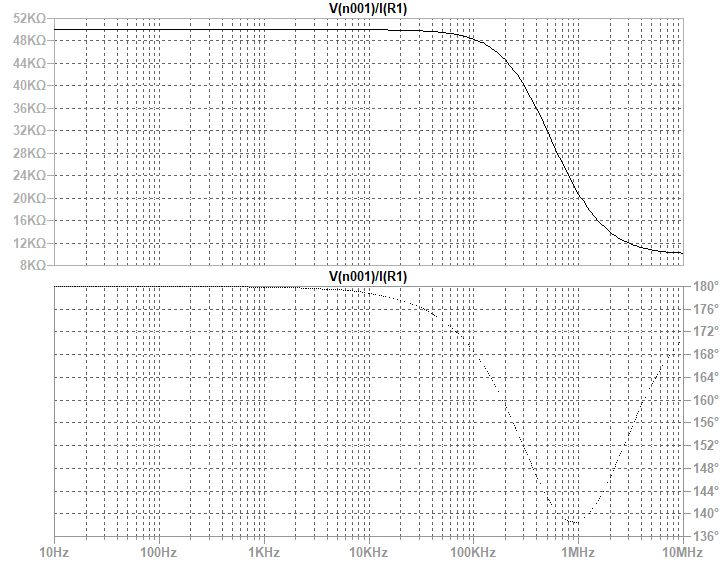
\includegraphics[scale=0.5]{../Ex1/iB/Resources1b/zinp1_sim_para}
\par\end{centering}
\caption{Simulación de impedancia de entrada para el caso 1, considerando una
capacidad parásita de 10(pF)}

\end{figure}

\begin{figure}[H]
\begin{centering}
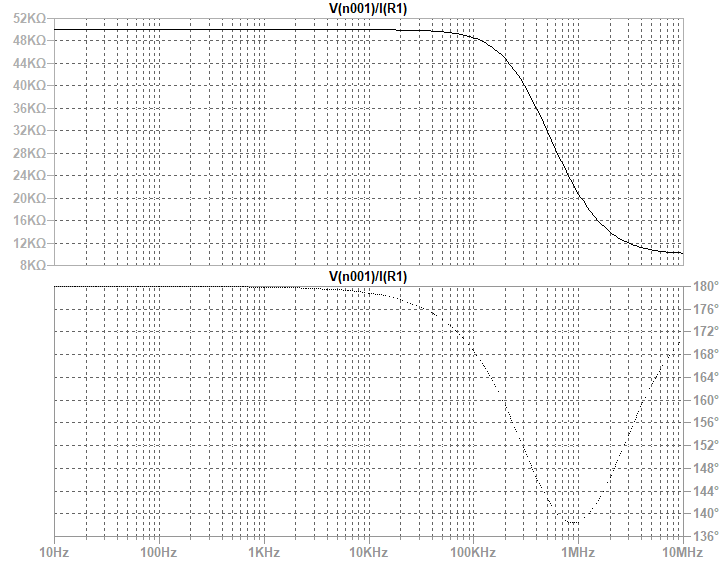
\includegraphics[scale=0.5]{../Ex1/iB/Resources1b/zinp2_sim_para}
\par\end{centering}
\caption{Simulación de impedancia de entrada para el caso 2, considerando una
capacidad parásita de 10(pF)}
\end{figure}

\begin{figure}[H]
\begin{centering}
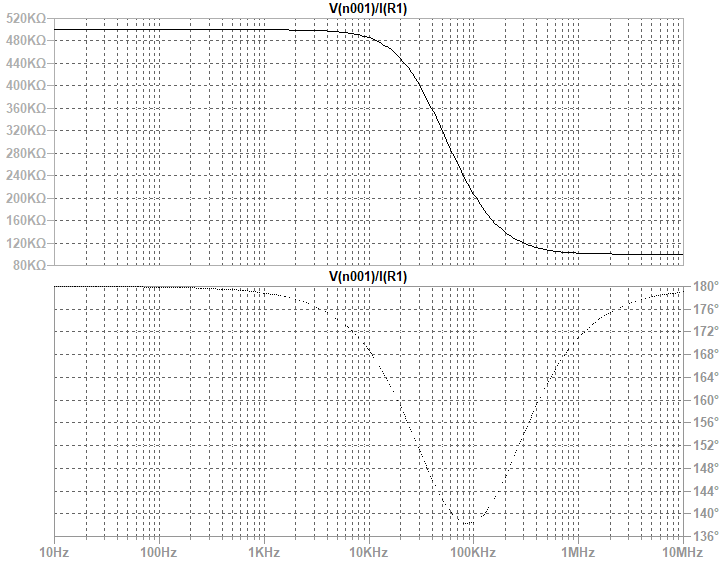
\includegraphics[scale=0.5]{../Ex1/iB/Resources1b/zinp3_sim_para}
\par\end{centering}
\caption{Simulación de impedancia de entrada para el caso 3, considerando una
capacidad parásita de 10(pF)}
\end{figure}

\subsection{Alinialidades}

\subsubsection{Saturación y polo dominante}

Teniendo en cuenta que la salida del Amplificador Operacional no podrá
ser en modulo mayor a $V_{cc}$, se calculó, como se explico en la
sección anterior, el máximo valor de la tensión de entrada dependiente
de la frecuecia de entrada, para el cual el circuito no satura.

\[
\left|H(f)\right|\times V_{in}=\frac{R_{4}\omega_{p}a_{0}\left(R_{1}+R_{2}\right)}{\left(R_{3}+R_{4}\right)\sqrt{4f^{2}\pi^{2}\left(R_{1}+R_{2}\right)^{2}+\left(R_{1}\omega_{p}a_{0}+\omega_{p}\left(R_{1}+R_{2}\right)\right)^{2}}}\times V_{in}\leq V_{cc}
\]

\[
V_{in}\leq\frac{Vcc\left(R_{3}+R_{4}\right)\sqrt{4\pi^{2}f^{2}\left(R_{1}+R_{2}\right)^{2}+\left(R_{1}\omega_{p}a_{0}+R_{1}\omega_{p}+R_{2}\omega_{p}\right)^{2}}}{R_{4}\omega_{p}a_{0}\left(R_{1}+R_{2}\right)}
\]

\[
V_{in}\leq2.4\cdot10^{-12}Vcc\sqrt{48,4\times10^{9}\pi^{2}f^{2}+2.2\cdot10^{21}}\,\,\,Caso\,1
\]

\[
V_{in}\leq1.3\cdot10^{-11}Vcc\sqrt{1,6\times10^{9}\pi^{2}f^{2}+2.2\cdot10^{21}}\,\,\,Caso\,2
\]

\[
V_{in}\leq2.4\cdot10^{-12}Vcc\sqrt{48,4\times10^{9}\pi^{2}f^{2}+2.2\cdot10^{23}}\,\,\,Caso\,3
\]

Observando estas ecuaciones, y graficandolas para cada caso, podemos
que en general, para grandes frecuencias, el efecto de saturación
no se hace presente debido al comportamiento pasabajos de el circuito
analizado.

\begin{figure}[H]
\begin{centering}
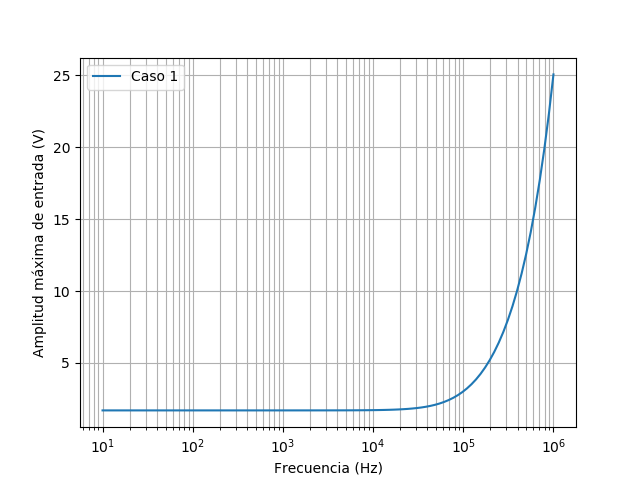
\includegraphics[scale=0.5]{../Ex1/iB/Resources1b/sat1}
\par\end{centering}
\caption{Tensión de entrada máxima respecto de la frecuencia de entrada para
que no ocurra saturación en el caso 1}

\end{figure}

\begin{figure}[H]
\begin{centering}
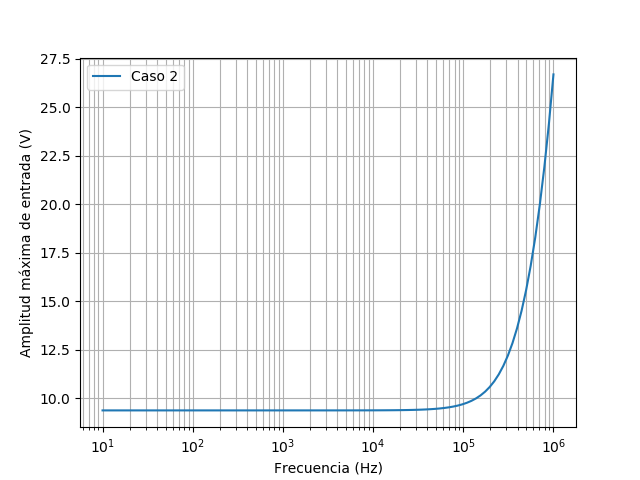
\includegraphics[scale=0.5]{../Ex1/iB/Resources1b/sat2}
\par\end{centering}
\caption{Tensión de entrada máxima respecto de la frecuencia de entrada para
que no ocurra saturación en el caso 2}
\end{figure}

\begin{figure}[H]
\begin{centering}
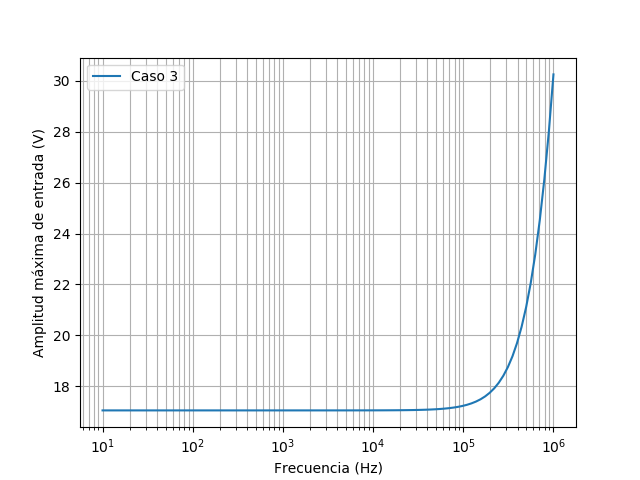
\includegraphics[scale=0.5]{../Ex1/iB/Resources1b/sat3}
\par\end{centering}
\caption{Tensión de entrada máxima respecto de la frecuencia de entrada para
que no ocurra saturación en el caso 3}
\end{figure}

\begin{figure}[H]
\begin{centering}
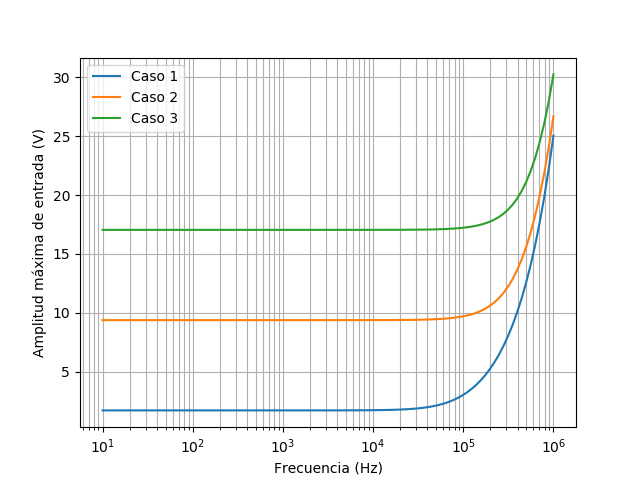
\includegraphics[scale=0.5]{../Ex1/iB/Resources1b/sat123}
\par\end{centering}
\caption{Tensión de entrada máxima respecto de la frecuencia de entrada para
que no ocurra saturación}
\end{figure}

\subsubsection{Slew Rate}

Por otro lado, se analizó el efecto \emph{Slew Rate }de la misma manera
que se lo hizo en la seccion anterior, es decir, $\frac{\partial V_{out}}{\partial t}\leq SR$,
por lo tanto, tenemos que, $v_{in}(t)=V_{p}sin(2\pi ft)$, por ende,
$V_{out}(t)=\left|H(f)\right|V_{p}2\pi f\,cos(2\pi ft+\phi(f))$.
A su vez, el coseno siempre es menor a 1, por ende;

\[
\frac{\partial V_{out}}{\partial t}\leq\left|H(f)\right|V_{p}2\pi f\leq SR
\]

\begin{equation}
\Rightarrow V_{p}\leq\frac{SR}{\left|H(f)\right|f2\pi}\label{eq:1_b_asd}
\end{equation}

Reemplazando en la inecuación (\ref{eq:1_b_asd}), tenemos que;

\[
V_{in}\leq\frac{SR\left(R_{3}+R_{4}\right)\sqrt{4\pi^{2}f^{2}\left(R_{1}+R_{2}\right)^{2}+\left(R_{1}\omega_{p}a_{0}+R_{1}\omega_{p}+R_{2}\omega_{p}\right)^{2}}}{2\pi R_{4}\omega_{p}a_{0}f\left(R_{1}+R_{2}\right)}
\]

\[
V_{in}\leq\frac{1.2\times10^{-12}SR\sqrt{48.2\times10^{9}\pi^{2}f^{2}+2.2\times10^{21}}}{\pi f}\,\,\,Caso\,1
\]

\[
V_{in}\leq\frac{6.6\times10^{-12}SR\sqrt{16\times10^{9}\pi f^{2}+2.2\times10^{21}}}{\pi f}\,\,\,Caso\,2
\]

\[
V_{in}\leq\frac{1.2\times10^{-12}SR\sqrt{48,4\times10^{9}\pi^{2}f^{2}+2.2\times10^{23}}}{\pi f}\,\,\,Caso\,3
\]

Si ahora reemplazamos para cada caso $SR=0,55836\left(\frac{V}{\mu s}\right)$
(como fue calculado en la sección anterior para el LM324), y graficamos
la amplitud de entrada máxima frente a la frecuencia de entrada, nos
quedan las Figuras \ref{1_b_23}, \ref{1_b_24}, \ref{1_b_25} y \ref{1_b_26}.

\begin{figure}[H]
\begin{centering}
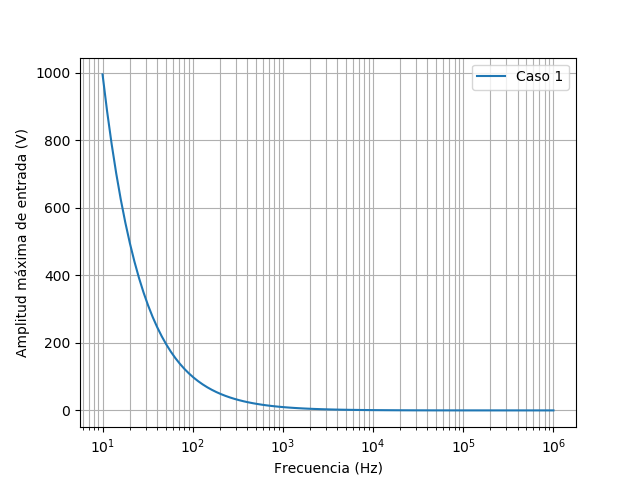
\includegraphics[scale=0.5]{../Ex1/iB/Resources1b/slewRate1}
\par\end{centering}
\caption{Tensión de entrada máxima respecto de la frecuencia de entrada para
que no ocurra \emph{Slew Rate} en el caso 1}
\label{1_b_23}
\end{figure}

\begin{figure}[H]
\begin{centering}
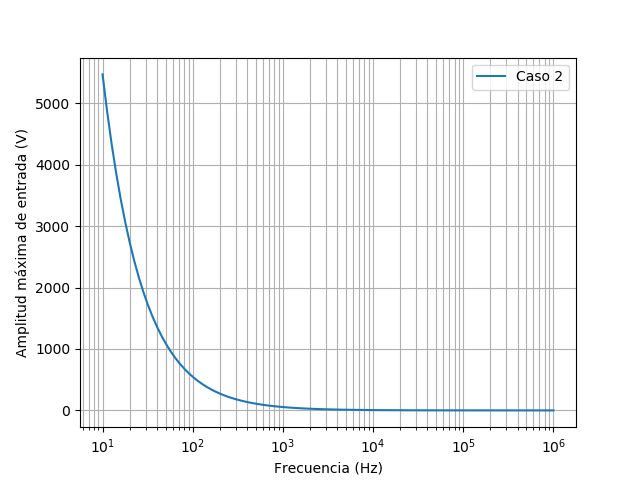
\includegraphics[scale=0.5]{../Ex1/iB/Resources1b/slewRate2}
\par\end{centering}
\caption{Tensión de entrada máxima respecto de la frecuencia de entrada para
que no ocurra \emph{Slew Rate} en el caso 2}
\label{1_b_24}
\end{figure}

\begin{figure}[H]
\begin{centering}
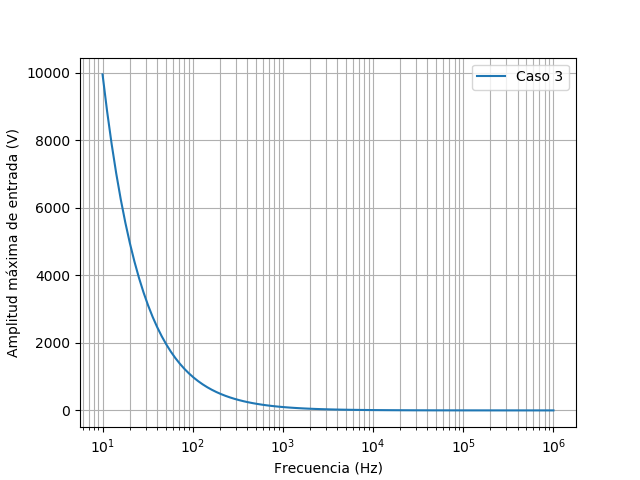
\includegraphics[scale=0.5]{../Ex1/iB/Resources1b/slewRate3}
\par\end{centering}
\caption{Tensión de entrada máxima respecto de la frecuencia de entrada para
que no ocurra \emph{Slew Rate} en el caso 3}
\label{1_b_25}
\end{figure}

\begin{figure}[H]
\begin{centering}
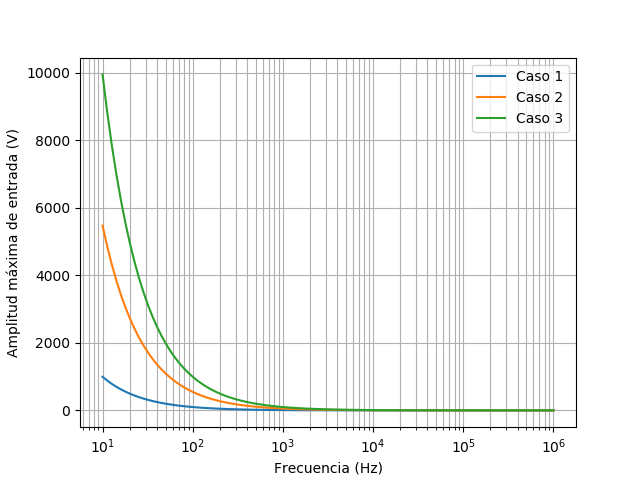
\includegraphics[scale=0.5]{../Ex1/iB/Resources1b/slewRate123}
\par\end{centering}
\caption{Tensión de entrada máxima respecto de la frecuencia de entrada para
que no ocurra \emph{Slew Rate}}
\label{1_b_26}
\end{figure}

\subsubsection{Conclusiones}

Por último, si tenemos en cuenta los efectos alinialies del \emph{Slew
Rate, }Saturación y \emph{Crossover Distortion} (el ultimo explicado
en la sección anterior), pueden ser armadas unas figuras mostradas
a continuación que muestran la máxima amplitud de una señal de entrada
a el circuito para cada caso, para que no se encuentren efectos aliniales
indeseados en las mediciones. Estas son las Figuras \ref{1_b_27},
\ref{1_b_28}, \ref{1_b_29} y \ref{1_b_30}.

\begin{figure}[H]
\begin{centering}
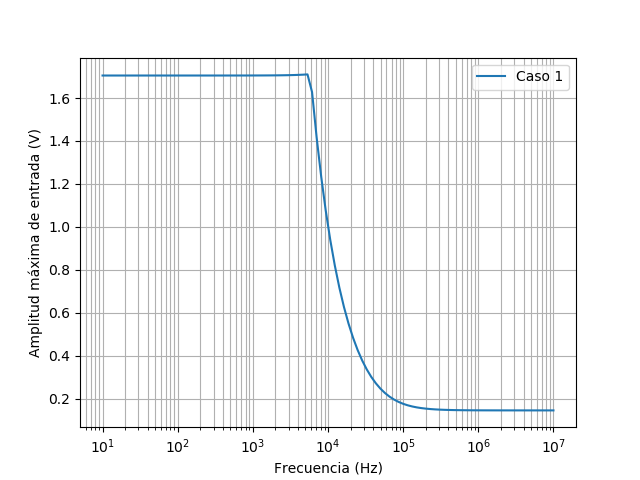
\includegraphics[scale=0.5]{../Ex1/iB/Resources1b/AmplMaxVsFreq1}
\par\end{centering}
\caption{Tensión máxima de entrada para que no ocurran alinialidades en el
caso 1}
\label{1_b_27}

\end{figure}

\begin{figure}[H]
\begin{centering}
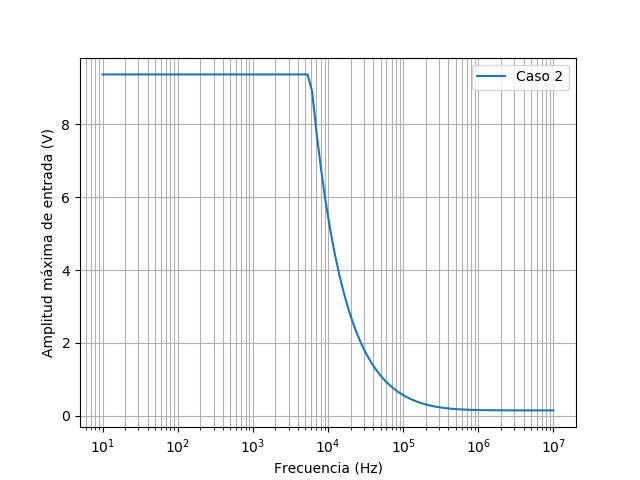
\includegraphics[scale=0.5]{../Ex1/iB/Resources1b/AmplMaxVsFreq2}
\par\end{centering}
\caption{Tensión máxima de entrada para que no ocurran alinialidades en el
caso 2}
\label{1_b_28}
\end{figure}

\begin{figure}[H]
\begin{centering}
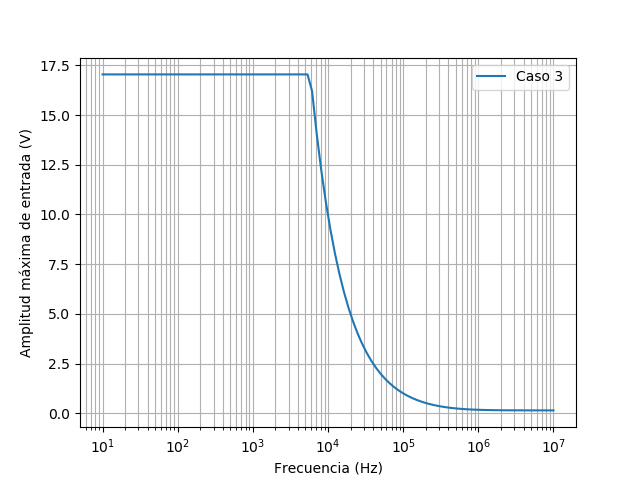
\includegraphics[scale=0.5]{../Ex1/iB/Resources1b/AmplMaxVsFreq3}
\par\end{centering}
\caption{Tensión máxima de entrada para que no ocurran alinialidades en el
caso 3}
\label{1_b_29}
\end{figure}

\begin{figure}[H]
\begin{centering}
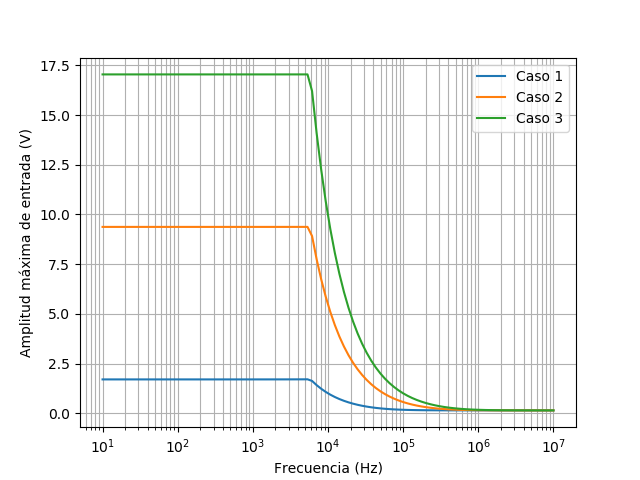
\includegraphics[scale=0.5]{../Ex1/iB/Resources1b/AmplMaxVsFreq123}
\par\end{centering}
\caption{Tensión máxima de entrada para que no ocurran alinialidades}
\label{1_b_30}
\end{figure}

\subsection{DC Sweep}

A continuación se procedio a realizar un DC Sweep para cada caso del
circuito, los resultados se muestran a continuación.

\begin{figure}[H]
\begin{centering}
\includegraphics[scale=0.3]{\string"../Ex1/iB/Resources1b/DC Sweep1_sim\string".png}\includegraphics[scale=0.3]{\string"../Ex1/iB/Resources1b/DC Sweep1_med\string".png}
\par\end{centering}
\caption{DC Sweep caso 1}
\end{figure}

\begin{figure}[H]
\begin{centering}
\includegraphics[scale=0.3]{\string"../Ex1/iB/Resources1b/DC Sweep2_sim\string".png}\includegraphics[scale=0.3]{\string"../Ex1/iB/Resources1b/DC Sweep2_med\string".png}
\par\end{centering}
\caption{DC Sweep caso 2}
\end{figure}

\begin{figure}[H]
\begin{centering}
\includegraphics[scale=0.3]{\string"../Ex1/iB/Resources1b/DC Sweep3_sim\string".png}\includegraphics[scale=0.3]{\string"../Ex1/iB/Resources1b/DC Sweep3_med\string".png}
\par\end{centering}
\caption{DC Sweep caso 3}
\end{figure}

Como se puede observar no hay grandes diferencias entre lo simulado
y lo medido.

\section{Conclusiones}

Es determinante tener en cuenta las alinialidades que provoca un Amplificador
Operacional, ya sea por saturación, \emph{Slew Rate }o por \emph{Crossover
Distortion, }ya que es muy importante para proceder a hacer mediciones
sobre los mismos. Estas alinialidades afectan en gran medida el comportamiento
del Amplificador Operacional, por lo tanto, si no se las tiene en
cuenta, es altamente probable que se cometan errores en mediciones
y resultados esperados.

Sumado a esto, es muy importante tener en cuenta los efectos de los
instrumentos de medición, ya sea Osciloscopios, Multimetros, Analizadores
de impedancias, etc. ya que las capacidades, inductancias y resistencias
parásitas afectan en gran medida el comportamiento de nuestro circuito.

Por último, se pudo observar que a un mismo \emph{Gain Bandwith Product
}(GBP), podemos cambiar nuestro circuito para que trabaje mas idealmente
a altas frecuencias. Es decir, que para un caso A con ganancia $\beta$,
y una frecuencia de corte $f_{0}$, y un caso B con ganancia $\beta^{'}$
y una frecuencia de corte $f_{0}^{'}$ , tenemos que $\beta^{'}\leq\beta$
y $f_{0}\leq f_{0}^{'}$, por lo tanto, podremos en el caso B trabajar
idealmente a mayores frecuencias, pero con menos ganancia, y por el
contrario, en el caso A trabajaremos con mas ganancia pero a menores
frecuencias.
